%%%%%%%%%%%%%%%%%%%%%%%%%%%%%%%%%%%%%%%%%%%%%%%%%%%%%%%%%%%%%%%%%%%%%%%%
%%%%%%%%%%%%%%%%%%%%%% Simple LaTeX CV Template %%%%%%%%%%%%%%%%%%%%%%%%
%%%%%%%%%%%%%%%%%%%%%%%%%%%%%%%%%%%%%%%%%%%%%%%%%%%%%%%%%%%%%%%%%%%%%%%%

%%%%%%%%%%%%%%%%%%%%%%%%%%%%%%%%%%%%%%%%%%%%%%%%%%%%%%%%%%%%%%%%%%%%%%%%
%% NOTE: If you find that it says                                     %%
%%                                                                    %%
%%                           1 of ??                                  %%
%%                                                                    %%
%% at the bottom of your first page, this means that the AUX file     %%
%% was not available when you ran LaTeX on this source. Simply RERUN  %%
%% LaTeX to get the ``??'' replaced with the number of the last page  %%
%% of the document. The AUX file will be generated on the first run   %%
%% of LaTeX and used on the second run to fill in all of the          %%
%% references.                                                        %%
%%%%%%%%%%%%%%%%%%%%%%%%%%%%%%%%%%%%%%%%%%%%%%%%%%%%%%%%%%%%%%%%%%%%%%%%

%%%%%%%%%%%%%%%%%%%%%%%%%%%% Document Setup %%%%%%%%%%%%%%%%%%%%%%%%%%%%

% Don't like 10pt? Try 11pt or 12pt
\documentclass[10pt]{article}
\usepackage{CJKutf8}
% This is a helpful package that puts math inside length specifications
\usepackage{calc}
\usepackage{pifont}
\usepackage{marvosym}
\usepackage{graphicx}
\usepackage{wrapfig}
%\usepackage{verbatim} 


% Simpler bibsection for CV sections
% (thanks to natbib for inspiration)
\makeatletter
\newlength{\bibhang}
\setlength{\bibhang}{1em}
\newlength{\bibsep}
 {\@listi \global\bibsep\itemsep \global\advance\bibsep by\parsep}
\newenvironment{bibsection}%
        {\vspace{-\baselineskip}\begin{list}{}{%
       \setlength{\leftmargin}{\bibhang}%
       \setlength{\itemindent}{-\leftmargin}%
       \setlength{\itemsep}{\bibsep}%
       \setlength{\parsep}{\z@}%
        \setlength{\partopsep}{0pt}%
        \setlength{\topsep}{0pt}}}
        {\end{list}\vspace{-.6\baselineskip}}
\makeatother

% Layout: Puts the section titles on left side of page
\reversemarginpar

%
%         PAPER SIZE, PAGE NUMBER, AND DOCUMENT LAYOUT NOTES:
%
% The next \usepackage line changes the layout for CV style section
% headings as marginal notes. It also sets up the paper size as either
% letter or A4. By default, letter was used. If A4 paper is desired,
% comment out the letterpaper lines and uncomment the a4paper lines.
%
% As you can see, the margin widths and section title widths can be
% easily adjusted.
%
% ALSO: Notice that the includefoot option can be commented OUT in order
% to put the PAGE NUMBER *IN* the bottom margin. This will make the
% effective text area larger.
%
% IF YOU WISH TO REMOVE THE ``of LASTPAGE'' next to each page number,
% see the note about the +LP and -LP lines below. Comment out the +LP
% and uncomment the -LP.
%
% IF YOU WISH TO REMOVE PAGE NUMBERS, be sure that the includefoot line
% is uncommented and ALSO uncomment the \pagestyle{empty} a few lines
% below.
%

%% Use these lines for letter-sized paper
%\usepackage[paper=letterpaper,
%           %includefoot, % Uncomment to put page number above margin
%            marginparwidth=0.7in,     % Length of section titles
%            marginparsep=.05in,       % Space between titles and text
%            margin=0.5in,               % 1 inch margins
%            includemp]{geometry}

% Use these lines for A4-sized paper
\usepackage[paper=a4paper,
            %includefoot, % Uncomment to put page number above margin
            marginparwidth=24mm,    % Length of section titles
            marginparsep=1mm,       % Space between titles and text
            margin=15mm,              % 25mm margins
            includemp]{geometry}

%% More layout: Get rid of indenting throughout entire document
\setlength{\parindent}{0in}

%% This gives us fun enumeration environments. compactitem will be nice.
\usepackage{paralist}
\usepackage[shortlabels]{enumitem}
% \usepackage[misc]{ifsym}
%% Reference the last page in the page number
%
% NOTE: comment the +LP line and uncomment the -LP line to have a page
%       numbers without the ``of ##'' last page reference)
%
% NOTE: uncomment the \pagestyle{empty} line to get rid of all page
%       numbers (make sure include foot is commented out above)
%
\usepackage{fancyhdr,lastpage}
\pagestyle{fancy}
%\pagestyle{empty}      % Uncomment this to get rid of page numbers
\fancyhf{}\renewcommand{\headrulewidth}{0pt}
\fancyfootoffset{\marginparsep+\marginparwidth}
\newlength{\footpageshift}
\setlength{\footpageshift}
          {0.1\textwidth+0.1\marginparsep+0.1\marginparwidth-2in}
\lfoot{\hspace{\footpageshift}%
       \parbox{3.5in}{\, \hfill %
                    \arabic{page} of \protect\pageref*{LastPage} % +LP
%                    \arabic{page}                               % -LP
                    \hfill \,}}

% Finally, give us PDF bookmarks
\usepackage{color,hyperref}
\definecolor{darkblue}{rgb}{0.0,0.0,0.3}
\hypersetup{colorlinks,breaklinks,
            linkcolor=darkblue,urlcolor=darkblue,
            anchorcolor=darkblue,citecolor=darkblue}

%%%%%%%%%%%%%%%%%%%%%%%% End Document Setup %%%%%%%%%%%%%%%%%%%%%%%%%%%%


%%%%%%%%%%%%%%%%%%%%%%%%%%% Helper Commands %%%%%%%%%%%%%%%%%%%%%%%%%%%%

% The title (name) with a horizontal rule under it
%
% Usage: \makeheading{name}
%
% Place at top of document. It should be the first thing.
\newcommand{\makeheading}[1]%
        {\hspace*{-\marginparsep minus \marginparwidth}%
         \begin{minipage}[t]{\textwidth+\marginparwidth+\marginparsep}%
                {\large \bfseries #1}\\[-0.15\baselineskip]%
                 \rule{\columnwidth}{1pt}%
         \end{minipage}}

% The section headings
%
% Usage: \section{section name}
%
% Follow this section IMMEDIATELY with the first line of the section
% text. Do not put whitespace in between. That is, do this:
%
%       \section{My Information}
%       Here is my information.
%
% and NOT this:
%
%       \section{My Information}
%
%       Here is my information.
%
% Otherwise the top of the section header will not line up with the top
% of the section. Of course, using a single comment character (%) on
% empty lines allows for the function of the first example with the
% readability of the second example.
\renewcommand{\section}[2]%
        {\pagebreak[2]\vspace{1\baselineskip}%
         \phantomsection\addcontentsline{toc}{section}{#1}%
         \hspace{0in}%
         \marginpar{
         \raggedright \scshape #1}#2}

% An itemize-style list with lots of space between items
\newenvironment{outerlist}[1][\enskip\textbullet]%
        {\begin{itemize}[#1]}{\end{itemize}%
         \vspace{-0.6\baselineskip}}

% An environment IDENTICAL to outerlist that has better pre-list spacing
% when used as the first thing in a \section
\newenvironment{lonelist}[1][\enskip\textbullet]%
        {\vspace{-\baselineskip}\begin{list}{#1}{%
        \setlength{\partopsep}{0pt}%
        \setlength{\topsep}{0pt}}}
        {\end{list}\vspace{-.6\baselineskip}}

% An itemize-style list with little space between items
% \newenvironment{innerlist}[1][\enskip\textbullet]%
\newenvironment{innerlist}[1][\enskip$\circ$]%
        {\begin{compactitem}[#1]}{\end{compactitem}}

% An environment IDENTICAL to innerlist that has better pre-list spacing
% when used as the first thing in a \section
\newenvironment{loneinnerlist}[1][\enskip\textbullet]%
        {\vspace{-\baselineskip}\begin{compactitem}[#1]}
        {\end{compactitem}\vspace{-.6\baselineskip}}

% To add some paragraph space between lines.
% This also tells LaTeX to preferably break a page on one of these gaps
% if a needed page break is nearby.
\newcommand{\blankline}{\quad\pagebreak[2]}

% Uses hyperref to link DOI
\newcommand\doilink[1]{\href{http://dx.doi.org/#1}{#1}}
\newcommand\doi[1]{doi:\doilink{#1}}


%%%%%%%%%%%%%%%%%%%%%%%% End Helper Commands %%%%%%%%%%%%%%%%%%%%%%%%%%%

%%%%%%%%%%%%%%%%%%%%%%%%% Begin CV Document %%%%%%%%%%%%%%%%%%%%%%%%%%%%

%\hyphenpenalty = 9999
\def\vs{\vspace{-0.1in}}
\begin{document}
% \makeheading{Curriculum Vitae\\ [0.3cm] TIEP HUU VU\quad~~~~~~\quad\quad\quad\quad\quad\quad\quad\quad\quad\quad\quad\quad\quad\quad{\small Last update: December 17, 2015}}



\newlength{\rcollength}\setlength{\rcollength}{3 in}
\vs

%% ==============================================================
\vspace{0.2in}

%\section{Research Background} % (fold)
%\label{sec:research_backg}
%\vspace{-0.25in}

%\begin{outerlist}
%  \item {\bf Graph Unsupervised Learning}: Graph Clustering/ Community Detection, Graph Representation Learning, Graph Contrastive Learning.
%  \item {\bf Graph Conformal Prediction:} Conformal Prediction for Node Classification.
%\end{outerlist}
% section research_backg (end)
%% =========  ==============================

\begin{CJK}{UTF8}{gbsn}
	
% \makeheading{Curriculum Vitae\\ [0.3cm] TIEP HUU VU\quad~~~~~~\quad\quad\quad\quad\quad\quad\quad\quad\quad\quad\quad\quad\quad\quad{\small Last update: December 17, 2015}}
\makeheading{CHEN Han \hfill {\small Last update: Feb 03, 2023}}


\section{contact\\information}
\begin{minipage}[l]{0.75\textwidth}
\begin{tabular}[t]{l@{}p{\textwidth-\rcollength}p{\rcollength}}
Tel: +86-13305014345\\
{\large\Letter} \texttt{E-mail:}\href{mailto:concyclics@qq.com}{concyclics@qq.com} 
\\
\texttt{Github:}\href{https://www.github.com/Concyclics}{www.github.com/Concyclics}\\
%\texttt{Gitee:}\href{https://www.gitee.com/Concyclics}{www.gitee.com/concyclics}\\
\texttt{Kaggle:}\href{https://www.kaggle.com/concyclics}{www.kaggle.com/concyclics} \\
\texttt{Address}: University Town Campus, Panyu District, \\
				\quad \quad \quad \quad \enspace South China University of Technology, Guangzhou, China\\												
\end{tabular}
\end{minipage}
\begin{minipage}[r]{0.5\textwidth}
\quad \quad \quad \quad \quad \enspace 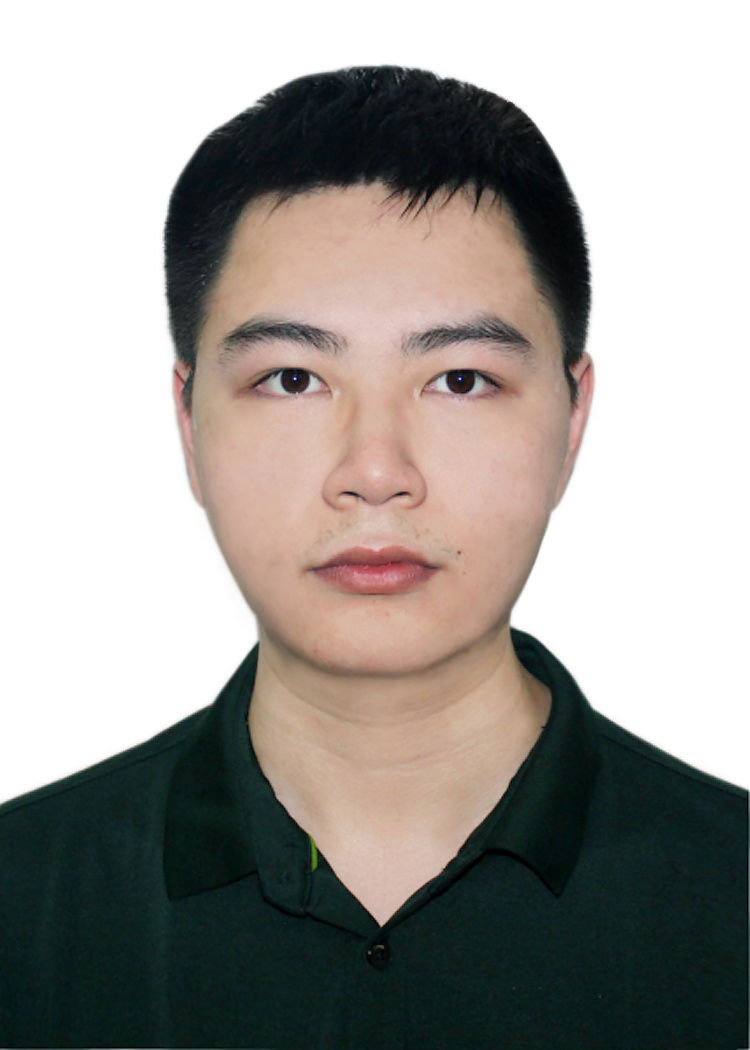
\includegraphics[width=0.25\textwidth]{face.jpg}\\
\end{minipage}
%% ==============================================================

%\section{Research Background} % (fold)
%\label{sec:research_backg}
%\vspace{-0.25in}

%\begin{outerlist}
%  \item {\bf Graph Unsupervised Learning}: Graph Clustering/ Community Detection, Graph Representation Learning, Graph Contrastive Learning.
%  \item {\bf Graph Conformal Prediction:} Conformal Prediction for Node Classification.
%\end{outerlist}
% section research_backg (end)
%% =========  ==============================
\vspace{-0.2in}
\section{education}
	\href{http://www.fzsz.net/}{\textbf{Fuzhou NO.3 High School}}, Fuzhou, China. \hfill 2016--2019
	\\
 \href{https://www.scut.edu.cn/en/}{\textbf{South China University of Technology (SCUT)}}, Guangzhou, China. \hfill 2019--2023
    \begin{innerlist}
        \item B.Eng., Software Engineering.
    \end{innerlist}
  
 %% =========  ==============================
\section{Technical Skills} % (fold)
\vspace{-0.2in}
\begin{outerlist}
  	\item {\it English}: IELTS(6.5), CET-4, CET-6.
  	\item {\it Programming Languages}: C/C++, Fortran, Python, MySQL, sqlite, \LaTeX.
  	\item {\it Programming skills}: intel oneapi, openblas, openmp, pthread, pytorch, keras.
  	\item {\it TestDemo Certificate}: \href{https://app.testdome.com/cert/bc443ba08d3442d1a4de9e7aea611dfa}{C++, TOP 10\%}, \href{https://app.testdome.com/cert/71e9426611324cce8a5dff69d23da9a5}{LINUX, TOP 10\%}, \href{https://app.testdome.com/cert/9af88d532837416f80620799c6fa1c9f}{PYTHON, TOP 10\%}
   	\item {\it Kaggle Certificate}: \href{https://www.kaggle.com/learn/certification/concyclics/data-visualization}{Data Visualization}, \href{https://www.kaggle.com/learn/certification/concyclics/intro-to-machine-learning}{Intro to Machine Learning}, \href{https://www.kaggle.com/learn/certification/concyclics/intro-to-deep-learning}{Intro to Deep Learning}, \href{https://www.kaggle.com/learn/certification/concyclics/intro-to-game-ai-and-reinforcement-learning}{Intro to Game AI and Reinforcement Learning}
  %\item {\it Technical Softwares}: MATLAB.
\end{outerlist}

%% =========  ==============================
\section{Honors \\and\\ Awards}
\vspace{-0.2in}
\begin{outerlist}
	\item \textbf{\textit{Silver Award (46th)}} ICPC Asia JiNan Regional Contest. \hfill 2021

	\item \textbf{\textit{Bronze Award (46th)}} ICPC Asia-East Continent Final. \hfill 2022

	\item \textbf{\textit{Silver Award (3rd)}} \\National College Students Algorithm Design\&Programming Challenge Contest\hfill 2022

	\item \textbf{National Scholarship} \hfill 2022

	\item \textbf{\textit{The First Prize Scholarship} Hong Ping Evergreen Fund}\\Student Science and Technology Innovation Competition scholarship\hfill 2022

	\item \textbf{\textit{Outstanding Contribution Award}} \\Extracurricular Academic Science and Technology Innovation\&Competition of 
	\\South China University of Technology\hfill 2022
	
	\item \textbf{\textit{Kaggle Dataset Expert}} \href{https://www.kaggle.com/concyclics}{Rank 181/63093} \hfill 2022

	\item \textbf{\textit{Kaggle Notebook Expert}} \href{https://www.kaggle.com/concyclics}{Rank 964/221587} \hfill 2022
\end{outerlist}


%% ================== block:  ==========================
\section{PROJECT\\EXPERIENCE}
\vspace{-0.2in}
\begin{outerlist}

\item {\it\textbf{Parallel Optimization Symmetric Matrix Solution with BBK Algorithm}}\\
	Mentor: \href{http://www2.scut.edu.cn/sse/2018/0614/c16789a270678/page.htm}{TANG Deyou}\hfill May-Dec. 2022\\
	\vspace{-0.1in}
	\begin{innerlist}
		\item Implemented the subroutine of solving symmetric matrix with bounded Bunch-Kaufman algorithm.
		\item Optimized the performance with openmp and using NEON intrinsics to improve parallelism and performance.
		\item Modified the cache-hit rate and parallelism during a column-swap part to achieve a 70\% total performance improvement.
	\end{innerlist}

\item {\it \textbf{Risk Management for Extreme Climate Disaster Chain in the Greater Bay Area}}\\
	Mentor: \href{http://www2.scut.edu.cn/sse/2019/0419/c16789a314444/page.htm}{TAO Qian}\hfill Mar.-July 2022\\
	\vspace{-0.1in}
	\begin{innerlist}
		\item Used Python libraries like Matplotlib, Plotly, and Pandas to perform correlation analysis, visualization analysis and doing some feature engineering according to the tropical cyclone measurement data from the China Meteorological Administration. 
		\item Predicted climate changes and estimated risks with GAT net.
	\end{innerlist}
 
\end{outerlist}

%% ================== block:  ==========================%

\section{EXCHANGE\\EXPERIENCE}
\vspace{-0.2in}
\begin{outerlist}
\item \textbf{Online Academic Program on Machine Learning, McGill University} \hfill Jan.-Feb. 2022\\
	\vspace{-0.1in}
	\begin{innerlist}
		\item Learned basic machine learning techniques and data analysis skill.
		\item Participated in competitions on Kaggle, e.g., image classification using CNN , English text classification using RNN, etc.
		\item Composed a proposal about the data analysis of consumption habits.
	\end{innerlist}
\end{outerlist}

% \makeheading{Curriculum Vitae\\ [0.3cm] TIEP HUU VU\quad~~~~~~\quad\quad\quad\quad\quad\quad\quad\quad\quad\quad\quad\quad\quad\quad{\small Last update: December 17, 2015}}


%% ==============================================================


%\section{Research Background} % (fold)
%\label{sec:research_backg}
%\vspace{-0.25in}

%\begin{outerlist}
%  \item {\bf Graph Unsupervised Learning}: Graph Clustering/ Community Detection, Graph Representation Learning, Graph Contrastive Learning.
%  \item {\bf Graph Conformal Prediction:} Conformal Prediction for Node Classification.
%\end{outerlist}
% section research_backg (end)
%% =========  ==============================

\begin{CJK}{UTF8}{gbsn}
	
% \makeheading{Curriculum Vitae\\ [0.3cm] TIEP HUU VU\quad~~~~~~\quad\quad\quad\quad\quad\quad\quad\quad\quad\quad\quad\quad\quad\quad{\small Last update: December 17, 2015}}
\makeheading{陈 涵 \hfill {\small 最近更新: 十二月 15, 2022}}


\section{联系方式}
\begin{minipage}[l]{0.74\textwidth}
\begin{tabular}[t]{l@{}p{\textwidth-\rcollength}p{\rcollength}}
Tel: +86-13305014345\\
{\large\Letter} \texttt{E-mail:}\href{mailto:concyclics@qq.com}{concyclics@qq.com} 
\\
\texttt{Github:}\href{https://www.github.com/Concyclics}{www.github.com/Concyclics}\\
\texttt{Gitee:}\href{https://www.gitee.com/Concyclics}{www.gitee.com/concyclics}\\
\texttt{Kaggle:}\href{https://www.kaggle.com/concyclics}{www.kaggle.com/concyclics} \\
\texttt{邮寄地址}: 广东省番禺区小谷围街道华南理工大学\\												
\end{tabular}
\end{minipage}
\begin{minipage}[r]{0.8\textwidth}
\begin{tabular}[t]{c@{}p{\textwidth-\rcollength}p{\rcollength}}
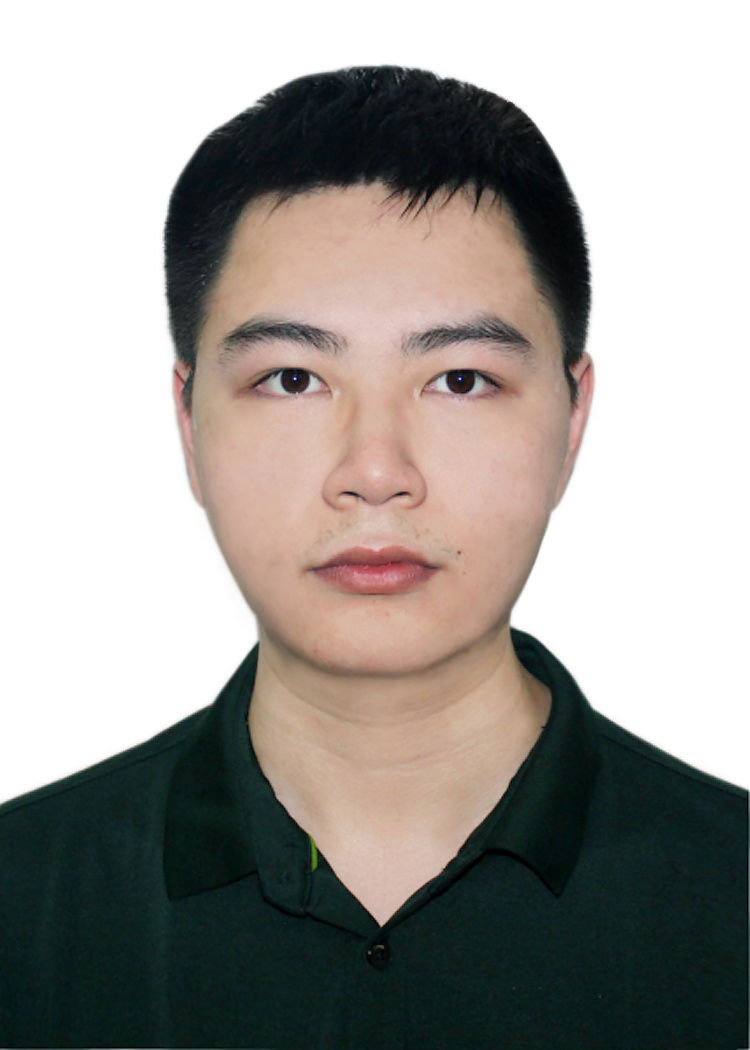
\includegraphics[width=0.2\textwidth]{face.jpg}\\

\end{tabular}
\end{minipage}
%% ==============================================================

%\section{Research Background} % (fold)
%\label{sec:research_backg}
%\vspace{-0.25in}

%\begin{outerlist}
%  \item {\bf Graph Unsupervised Learning}: Graph Clustering/ Community Detection, Graph Representation Learning, Graph Contrastive Learning.
%  \item {\bf Graph Conformal Prediction:} Conformal Prediction for Node Classification.
%\end{outerlist}
% section research_backg (end)
%% =========  ==============================
\section{教育经历}
	\href{http://www.fzsz.net/}{\textbf{福建省福州第三中学}}, 福建省福州市. \hfill 2016--2019
	\\
    \href{https://www.scut.edu.cn/en/}{\textbf{华南理工大学}},\href{http://www2.scut.edu.cn/sse/}{\textbf{软件学院}},广东省广州市. \hfill 2019--2023

%% =========  ==============================
\section{获奖荣誉}
\vspace{-0.3in}
\begin{outerlist}

\item 华南理工大学\textbf{\textit{优秀共青团员}} \hfill 2019\&2021
\item \textbf{\textit{银牌}} 第46届国际大学生程序设计竞赛(ACM-ICPC) \hfill 2021
\item \textbf{\textit{铜牌}} 第46届国际大学生程序设计竞赛亚洲区决赛(ACM-ICPC EC final) \hfill 2022
\item \textbf{国家奖学金} \hfill 2022
%\item \textbf{\textit{顽强拼搏奖}} 第46届国际大学生程序设计竞赛亚洲区决赛 \hfill 2022
\item \textbf{\textit{银牌}} 第三届全国大学生算法设计与编程挑战赛 (秋季赛) \hfill 2022
\item \textbf{\textit{铜牌}} 第三届全国大学生算法设计与编程挑战赛 (冬季赛) \hfill 2022
\item \textbf{\textit{铜牌}} 第三届全国大学生算法设计与编程挑战赛 (夏季赛) \hfill 2022
\item \textbf{\textit{一等奖}} “宏平长青基金”学生科技创新竞赛奖学金\hfill 2022
\item  \textbf{\textit{银牌}} 集美大学第八届程序设计竞赛. \hfill 2022
\item \textbf{\textit{杰出贡献奖}} 华南理工大学课外学术科技创新竞赛成果\hfill 2022
\item \textbf{\textit{Kaggle 数据专家(Dataset Expert)}} \href{https://www.kaggle.com/concyclics}{排名 181/63093} \hfill 2022
\item \textbf{\textit{Kaggle 代码专家(Notebook Expert)}} \href{https://www.kaggle.com/concyclics}{排名 964/221587} \hfill 2022
\end{outerlist}


%% ================== block:  ==========================
\vspace{0.1in}

%% ================== block:  ==========================
\section{项目经历} % (fold)
\label{sec:technical_ski}
\vspace{-0.3in}
\begin{outerlist}

\item {\it 粤港澳大湾区极端天气气候灾害链的风险管控与应对} \hfill 2022/03-2022/07\\
 	项目编号: 2019YFC1510400\\
 	工作内容: 气象数据分析和图注意力网络研究\\ 
 	单位: 	华南理工大学软件学院软件服务工程与云计算团队陶乾实验室\\
 	导师: 陶乾
 	
 \item {\it 对称矩阵函数求解之BBK(rook)算法} \hfill 2022/04-12\\
 	工作内容: 针对华为鲲鹏处理器实现LAPACK数学库中对称矩阵求解BBK算法\\
 	对应{$sysv\_rk/sysv\_rook$}单双精度实复数四种数据类型的接口并进行多线程并行性能优化和SIMD指令集性能优化\\
 	单位:  	华为鲲鹏计算\\
 	导师: 汤德佑

\end{outerlist}



%% ================== block:  ==========================%

\section{专业技能} % (fold)
\label{sec:technical_ski}
\vspace{-0.3in}
\begin{outerlist}
  \item {\it 编程语言}: C/C++, Python, Fortran, MySQL, sqlite, \LaTeX, markdown.
  \item {\it 编程技能}:intel oneapi, openblas, openmp, pthread, pytorch, keras. 
  \item {\it 工业和信息化部人才交流中心}: 工业和信息化人才专业知识测评证书——C语言编程高阶
  \item {\it TestDemo 编程技能认证}: \href{https://app.testdome.com/cert/bc443ba08d3442d1a4de9e7aea611dfa}{C++, TOP 10\%}, \href{https://app.testdome.com/cert/71e9426611324cce8a5dff69d23da9a5}{LINUX, TOP 10\%}, \href{https://app.testdome.com/cert/9af88d532837416f80620799c6fa1c9f}{PYTHON, TOP 10\%}
\item {\it Kaggle 课程认证}: \href{https://www.kaggle.com/learn/certification/concyclics/data-visualization}{数据可视化}, \href{https://www.kaggle.com/learn/certification/concyclics/intro-to-machine-learning}{机器学习}, \href{https://www.kaggle.com/learn/certification/concyclics/intro-to-deep-learning}{深度学习}, \href{https://www.kaggle.com/learn/certification/concyclics/intro-to-game-ai-and-reinforcement-learning}{强化学习}

  \item {\it 英语认证水平}: CET-4, CET-6 IELTS(6.5).
\end{outerlist}


\end{CJK}
\end{document}